\renewcommand{\imagepath}{../30-mot/img}

\chapter{The 3-dimensional Magneto-optical Trap}
\epigraph{When is Your First MOT Due?}{protyre.co.uk}

\todo{TODO: make spectroscopic notation non-italic}

\section{Laser Cooling with Magneto-optical Traps}
\todo{History (Haensch, Earnshaw), examples, Nobel Prize 1997.}

Laser light exerting a force onto an atom is the underlying mechanism of laser cooling. There are different implementations of laser cooling, each one making use of a different way light can interact with atoms: Doppler-cooling techniques on the one hand, as e.g.\ used in magneto-optical traps, are limited by the spontaneous decay of excited states regarding the achievable temperature. Sub-Doppler-cooling techniques, on the other hand, circumvent this limit using a variety atom-light interactions, such as the optical dipole trap, Raman sideband cooling or Sisyphus cooling~\cite{foot_atomic_2005}.

The rest of this section is covering the theory of magneto-optical traps and the implementation of the 3-dimensional magneto-optical trap of the FermiQP demonstrator experiment. The explanations closely follow the respective chapters in~\cite{foot_atomic_2005} and~\cite{metcalf_laser_1999}.

\subsection*{Light scattering on atoms}
Electromagnetic waves carry momentum $\vec p = \hbar k$, which is directed into their propagation direction and depends on their wavelength $\lambda = \frac{2\pi}{k}$. When laser light scatters on atoms, a momentum transfer between the photons of the laser and the atoms takes place. The total transfer can be broken down into two parts: the absorption of laser photons where the atoms acquire momentum $\hbar \vec k$ per photon, and the spontaneous emission of photons where the atoms lose $\hbar \vec k_\text{emitted}$ per photon:
\begin{align}
    \vec p_\text{after} &= \vec p_\text{before} + \hbar \vec k + \hbar \vec k_\text{emitted}
\end{align}
The latter, however, averages to zero over many scattering events as photons are emitted into random directions. In this way, atoms loose momentum over many scattering events, if the propagation of the light and the atom movement are in opposite directions:
\begin{align}
    \Braket{\vec p_\text{after} - \vec p_\text{before}} = \Braket{\hbar \vec k} + \underbrace{\Braket{\hbar \vec k_\text{emitted}}}_{=0}
\end{align}
As visualized in figure~\ref{fig:light_scattering_momentum_transfer}, the atoms are decelerated opposite the direction of laser propagation, corresponding to cooling of the atoms.

\begin{figure}    
    \centering
    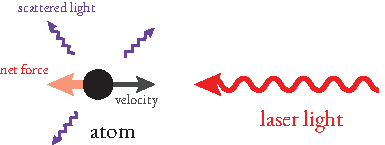
\includegraphics[]{\imagepath/light_scattering_momentum_transfer/light_scattering_momentum_transfer.pdf}
    \caption{Schematic of momentum transfer from the laser against the atom movement direction. The momenta of the scattered photons, originating from spontaneous in random directions, averages to zero.}\label{fig:light_scattering_momentum_transfer}
\end{figure}

The rate at which this happens is determined by the fraction $\rho_{ee}$ of atoms in the excited state when light of wavelength $\omega_\text{laser}$ and intensity $I$ is shone in:
\begin{align}
    R_\text{scatter} = \Gamma \rho_{ee}
\end{align}
with the rate $\Gamma$ of spontaneous decays from the excited state into the ground state. The scattering force which corresponds to the decrease of momentum of the atoms is hence
\begin{align}
    \vec F_\text{scatter} = R_\text{scatter} \hbar \vec k = \Gamma \rho_{ee} \hbar \vec k.
\end{align}

The light-atom interaction process can be described semi-classically understanding the light as a classical electromagnetic wave, but describing the dynamics within the atom using the quantum mechanical optical Bloch equations, according to which the steady-state population of the excited state amounts to
\begin{align}
    \rho_{ee} = \frac{s_0/2}{1 + s_0 + {\left(\frac{2\delta}{\Gamma}\right)}^2},
\end{align}
with the saturation parameter $s_0 = \frac{I}{I_s} = \frac{2\Omega^2}{\Gamma^2}$, the Rabi frequency $\Omega \propto \sqrt{I}$, and the detuning $\delta$. The detuning is the deviation of the laser frequency from the transition frequency, as seen by the atom considering the Doppler shift stemming from its velocity $\vec v$ with respect to the propagation direction $\vec k$ of the laser:
\begin{align}
    \delta &= \overbrace{\omega_\text{laser} - \vec k \vec v }^\text{apparent laser frequency}- \omega_\text{transition} \\
    \nonumber & = \omega_\text{laser}  - \omega_\text{transition} - kv \cos \theta
\end{align}
with the angle $\theta$ between the atoms' velocity and the propagation direction of the light.

\begin{figure}
    \centering
    \caption{Scattering force as a function of speed against the laser direction for different values of the detuning $\delta_\text{laser}$.
    \todo[inline]{add figure}
    }\label{fig:scattering_force_vs_velocity}
\end{figure}

Figure~\ref{fig:scattering_force_vs_velocity} shows how the scattering force depends on the velocity of the atoms. The force is maximal for velocities where Doppler shift $\vec k \vec v$ cancels out the laser detuning $\delta_\text{laser} = \omega_\text{laser} - \omega_\text{transition}$. Deceleration of atoms happens with red laser detuning $\delta_\text{laser} < 0$ as the light is resonant for atoms moving against the laser propagation direction. These atoms sense the light scattering force against their direction of movement; atoms moving in the other direction do not sense the scattering force (see figure~\ref{fig:scattering_force_detuning}).

\begin{figure}
    \centering
    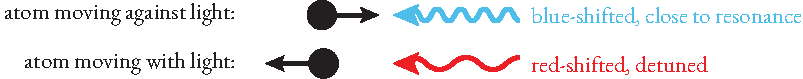
\includegraphics[]{\imagepath/scattering_force_detuning/scattering_force_detuning.pdf}
    \caption{Atoms moving against the direction of laser propagation see the laser light blue-shifted, atoms moving in the other direction see it red-shifted. For negative laser detuning ($\delta_\text{laser} < 0$) the former sense the light as it is close to resonance, the latter do not sense it as it is far detuned for them.}\label{fig:scattering_force_detuning}
\end{figure}

\paragraph*{Doppler limit} While the momentum gained by spontaneous emission of photons averages to zero, the square of momentum $\vec p_\text{after decay}^2$ gained from the spontaneous decays does not. This means that the atom is always left with a finite amount of kinetic energy from the recoil of emitted photons. The magnitude of this leftover energy is related to the decay rate $\Gamma$ and is called the Doppler limit:
\begin{align}
    k_B T_D = \frac{\hbar \Gamma}{2}
\end{align}
Laser cooling techniques using spontaneous emission of photons, by principle, cannot provide cooling below this limit (neglecting any coincidental sub-Doppler cooling effects)~\cite{foot_atomic_2005}.
\todo{mention recoil limit}


\subsection*{Magneto-optical Traps}
Magneto-optical traps use light scattering on atoms in order to cool and spatially confine atoms. They have become a standard tool in ultracold neutral atom experiments over the last decades.

\paragraph{Optical molasses} Magneto-optical traps make use of the optical molasses technique for slowing down atoms. As discussed above, light scattering provides a decelerating force opposite the direction of laser beams for red detuning. By using three pairs of counter-propagating laser beams, one pair in each spatial degree of freedom, atoms are decelerated in each direction. For an atom of speed $v \ll \frac{\Gamma}{k}$, travelling at an angle $\theta$ with respect to the  counter-propagating beams with wave number $k$, the scattering force in this direction can be linearized as as friction force
\begin{equation}
    \begin{split}
        F &= F(\omega_\text{laser} - \omega_\text{transition} - kv \cos \theta) - F(\omega_\text{laser} - \omega_\text{transition} + kv \cos \theta) \\
        &\approx - 2 \pdv{F}{\omega} k v \cos \theta \equiv -\alpha v \cos \theta
    \end{split}
\end{equation}
with damping $\alpha = 2k \pdv{F}{\omega}$\footnote{For $s_0 \ll 1$, the damping coefficient can be approximated as $\alpha  = 4 \hbar k^2 s_0 \frac{-2\delta/\Gamma}{{\left(1+{{(2\delta/\Gamma)}}^2\right)}^2}$~\cite{foot_atomic_2005}.}~\cite{foot_atomic_2005}. The velocity-dependence of the optical molasses deceleration force is depicted in figure~\ref{fig:optical_molasses_force}.

\begin{figure}
    \caption{Scattering force in optical molasses as a function of velocity. Due to the Doppler shift, only fast atoms (close to resonance) sense the scattering force. Here, the detuning was set to $\delta = -\Gamma/2$.
    \todo[inline]{add figure}
    }
    \label{fig:optical_molasses_force}
\end{figure}

\paragraph{Spatial confinement} For spatial confinement of atoms the Zeeman effect is exploited which shifts the energy levels of magnetic sublevels of spin or orbital angular momentum states under the influence of an external magnetic field. This energy shift with respect to a situation without a magnetic field, where the magnetic sublevels are degenerate, amounts to
\begin{align}
    \Delta E(m) = g \mu_B m B
\end{align}
with the Landé factor $g$, the Bohr magneton $\mu_B$, the magnetic field $B$ and the magnetic quantum number $m$. Applying a magnetic gradient, the transition frequencies between two magnetic sublevels $m$ and $m'$ becomes position-dependent:
\begin{equation}
    \begin{split}\label{eq:omega_transition_zeeman}
      \omega_\text{transition}(r) &= \omega_\text{transition} + \frac{\Delta E(r)}{\hbar} \\  
      &= \omega_\text{transition} + \frac{g \mu_B}{\hbar} \dv{B}{r} r \equiv \omega_\text{transition} + \beta r
    \end{split}
\end{equation}
Hence also the detuning between the laser light and the driven transition becomes position-dependent which allows for spatially varying scattering forces.

In order to create a confining trap, laser beams and magnetic gradients are calibrated such that the atoms sense restoring forces towards a center point when they move away from there. This means that on opposite sides of the trap, these restoring forces must point in opposite directions. One achieves this by clever use of the magnetic gradient and the polarization-dependent selection rules for transitions between magnetic sublevels, as visualized in figures~\ref{fig:restoring_on_opposite_sides_schematic} and~\ref{fig:detuning_and_selection_rules_schematic}:
\begin{itemize}
    \item Due to the magnetic gradient, the magnetic field has different sign on opposite sides of the trap center, hence also the Zeeman shifts $\Delta E$ have different sign for the transitions $\Delta m = +1$ and $\Delta m = -1$. This also means that on each side only one of these transitions is close to resonance with the laser light.
    \item $\sigma^+$ light (light with right helicity with respect to the atoms' quantization axis) can only drive transitions with $\Delta m = +1$, $\sigma^-$ light (left helicity) can only drive transitions with $\Delta m = -1$. In each pair of counter-propagating beams, one of the beams has $\sigma^+$ and one has $\sigma^-$ polarization, such that on each side the atoms only see the beam propagating towards the trap center.
\end{itemize}

\begin{figure}
    \centering
    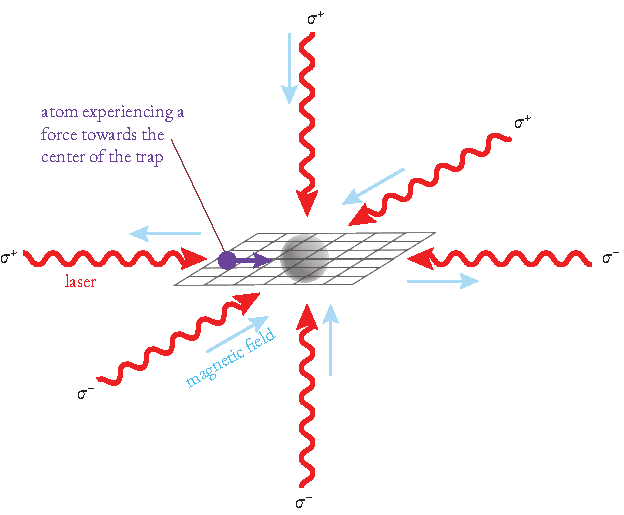
\includegraphics[]{\imagepath/restoring_on_opposite_sides_schematic/restoring_on_opposite_sides_schematic.pdf}
    \caption{Two-dimensional schematic of creation of restoring forces: Due to the magnetic gradient and the Zeeman effect, on each side of the trap, different transitions between magnetic sublevels are on resonance. Assigning different helicity of circular polarization to counter-propagating lasers, atoms only sense a scattering force in the direction of the trap center.}\label{fig:restoring_on_opposite_sides_schematic}
\end{figure} 

\begin{figure}
    \centering
    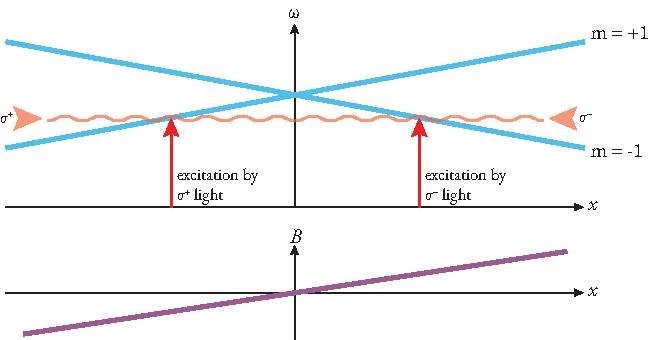
\includegraphics[]{\imagepath/detuning_and_selection_rules_schematic/detuning_and_selection_rules_schematic.pdf}
    \caption{One-dimensional schematic of selection rules and detunings of the laser beams: On both sides of the trap different transitions between magnetic sublevels are resonant with the red-detuned trap light. Due to the polarization-dependent selection rules, only one of the two counter-propagating beams is resonant on each side of the trap which sets the direction of momentum transfer between the light and the atoms. E.g. on the left center, the $\Ket{m = +1}$ state is closer to resonance. Only the $\sigma^+$ light coming from the left can excite this state, hence atoms on the left of the trap mostly acquire moment to the right, i.e. the trap center.
    \todo[inline]{Make m italic}
    }
    \label{fig:detuning_and_selection_rules_schematic}
\end{figure}

Note that the helicity of the polarization is given with respect to the (arbitrary, but fixed) quantization axis of the atoms. As the laser beams in each pair counter-propagate, one of them points to in and one against the quantization axis. The circular polarization with respect to their respective propagation direction is hence the same for both laser beams in a pair (both $\sigma^+$ or both $\sigma^-$, depending on the gradient field).


Similarly to the optical molasses consideration, in the magneto-optical trap the scattering forces can be linearized \todo{Under which condition?} (here again for one dimension)~\cite{foot_atomic_2005}:
\begin{equation}
    \begin{split}
        F_\text{MOT} &= F_{\sigma^+}(\omega_\text{laser} - \omega_\text{transition}(r) - kv \cos \theta) + F_{\sigma^-}(\omega_\text{laser} - \omega_\text{transition}(r) + kv \cos \theta)\\
        &= -2 \pdv{F}{\omega} k\cos \theta v + 2 \pdv{F}{\omega_0} \beta r  \equiv - \alpha \cos \theta v - \frac{\alpha \beta}{k} r
    \end{split}
\end{equation}
This shows how a magneto-optical trap combines the friction force $- \alpha v$ for slowing down atoms and the trapping force $- \frac{\alpha \beta}{k} z$ confining the atoms to a trap center.

\todo{Maybe add 3D plot with v, z, F axes.}

\paragraph{Characteristic quantities}
Important technical quantities that need to be adjusted for optimizing the performance of a MOT include:
\begin{itemize}
    \item laser intensities $I_\text{cooler}$ and $I_\text{repumper}$
    \item laser detunings with respect to the transition wavelength $\delta_\text{cooler}$ and $\delta_\text{repumper}$
    \item the angle $\theta$ of the atomic beam with respect to the cooling laser beams
    \item magnetic gradient $\pdv{B}{r}$
\end{itemize}

These quantities might also be varied over one trapping cycle, e.g. for compressing the trap and cooling the atoms further down by decreasing the laser intensity and the laser detuning and increasing the magnetic gradient.

The magneto-optical trap can be benchmarked by, among others, the following quantities:
\begin{itemize}
    \item The radius $r_\text{max}$ of the trapping region where the atoms are slowed  is on the order of the size of the trapping beams: $r_\text{max} \approx w$. The trap size is also limited by the distance $r_\text{resonance}$ from the trap center where the trapping beams become resonant due to the Zeeman shift (cf. equation \ref{eq:omega_transition_zeeman}): $\omega_\text{laser} - \omega_\text{transition} - \vec k \vec v = \frac{g \mu_B}{\hbar} \pdv{B}{r} r_\text{resonance}$. At larger distances from the trap, the trapping light is blue detuned and thus accelerating, hence slowing of atoms only occurs within a distance of $r_\text{resonance}$. In a one-dimensional consideration, one can deduce a maximum speed at which atoms entering the trap can still be on resonance~\cite{tiecke_high-flux_2009}:
    \begin{align}
        v_\text{max} = \frac{1}{k \cos \theta}\left(\omega_\text{laser} - \omega_\text{transition} - \frac{g \mu_B}{\hbar} \pdv{B}{r} r_\text{resonance}\right)
    \end{align}
    Given that the slowing force is large, one can assume that, on the way towards the trap center, the atoms are kept on resonance with the (due to the magnetic gradient) ever less detuned trapping light. In this case, $v_\text{max}$ can be used to estimate the capture velocity of the trap~\cite{tiecke_high-flux_2009}.
    \item The loading rate characterizes how many atoms can be trapped per time unit. It depends on the trap geometry, the flux rate and the velocity distribution of the incoming atoms, the applied gradients, laser powers, detunings of the cooling and repumping light, collisions among the trapped atoms, and many more. Due to these complex dependencies, the loading rate needs to be characterized experimentally.
    \item The temperature of the atoms in the trap. It usually in the order of magnitude above the Doppler temperature $T_D$\todo{add citation}.
    \item Regarding the trap as a harmonic oscillator, one can quantify the atom oscillation frequency $\omega_\text{MOT} = \frac{\alpha}{m}$, oscillation damping rate $\Gamma_\text{MOT} = \sqrt{\frac{\alpha \beta}{km}}$, and atom trap restoring time $t_\text{restore} = \frac{2\Gamma_\text{MOT}}{\omega_\text{MOT}^2}$ with atom mass $m$~\cite{metcalf_laser_1999}.
\end{itemize}

\paragraph{Relevant transitions in alkali atoms}
\sloppy For cooling alkali atoms in a magneto-optical trap, transitions between electronic levels $J_\text{g}$ and $J_\text{g} + 1$ are used. The cooling transition can be imple\-mented between hyperfine states $\KetSpaced{J = J_\text{g}, F = I + J_\text{g}}$ (the highest $F$ in the $J_\text{g}$ manifold), and $\KetSpaced{J = J_\text{g} + 1, F= I + J_\text{g} + 1}$. This ensures that all decays bring the atom down into the original $\KetSpaced{J = J_\text{g}, F = I + J_\text{g}}$ state due to the selection rule $\Delta F \in \{-1, 0, 1\}$.

If, however, the atom is excited into the $\KetSpaced{J = J_\text{e}, F = F_\text{g}}$ state due to a non-zero matrix element for this transition, it can also fall back into the $\KetSpaced{J = J_\text{e}, F = I + J_\text{g} - 1}$ state. In this case, it would not be subject to cooling anymore as this state is dark to the cooling transition. To combat this, a repumper laser beam is shone in in addition to the cooler beam. This beam addresses the transition $\KetSpaced{J = J_\text{g}, F = I + J_\text{g} - 1} \rightarrow \KetSpaced{J = J_\text{g} + 1, F = I + J_\text{g}}$ from where they can decay back into the ground state of the cooling transition which brings them back into the cooling cycle~\cite{metcalf_laser_1999}.

These cooling and repumping cascades are summarized in equations~\eqref{eq:cooler_cascade} and~\eqref{eq:repumper_cascade}:
\begin{align}
    \label{eq:cooler_cascade}\text{cooler:}~~~~~ & \KetSpaced{J_\text{g},I + J_\text{g}} \underset{\text{cooler}}{\longrightarrow} \KetSpaced{J_\text{g} + 1, I + J_\text{g} + 1} \rightsquigarrow  \KetSpaced{J_\text{g}, I + J_\text{g}}\\
    \label{eq:repumper_cascade}\text{repumper:}~~~~~ & \KetSpaced{J_\text{g} + 1, I + J_\text{g}} \rightsquigarrow \KetSpaced{J_\text{g}, I + J_\text{g} - 1}  \underset{\text{repumper}}{\longrightarrow} \KetSpaced{J_\text{g} + 1, I + J_\text{g}} \rightsquigarrow  \KetSpaced{J_\text{g}, I + J_\text{g}}
\end{align}
with notation being $\KetSpaced{J, F}$.

\begin{figure}
    \caption{Exemplary schematic of the cooling and repumping scheme in an alkali atom}\label{fig:cooler_repumper_in_alkali}
\end{figure}
\todo{Check with other source}


\section{Magneto-optical Traps with Lithium}
3-dimensional magneto-optical traps for lithium usually operate on the D$_2$ line, i.e.~between the $^2\text{S}_{1/2}$ and $^2\text{P}_{3/2}$ manifolds, as in the implementation in the FermiQP demonstrator. Since the first implementation with lithium in the early 1990s \cite{kawanaka_decay_1993}, they have become a standard part of ultracold lithium experiments, namely for experiments with fermionic~\cite{duarte_all-optical_2011,omran_microscopic_2015} and bosonic~\cite{kawanaka_decay_1993,schunemann_magneto-optic_1998} lithium as well as for isotope mixtures \cite{mewes_simultaneous_1999, hilker_laser_2012,kerkmann_novel_2019} and species mixtures \cite{ladouceur_compact_2009,tiecke_high-flux_2009,chen_lithium-cesium_2021}. [[TODO add streck 2002]]

For D$_2$ line traps for fermionic lithium, the energy splitting between the two ground state hyperfine manifolds $\KetSpaced{J=1/2, F=1/2}$ and $\KetSpaced{J=1/2, F=3/2}$ is \SI{228}{\mega\hertz}, which sets the difference in frequency for the cooler and repumper laser beams. The cooler addresses the transition $\Ket{^2\text{S}_{1/2}, F = 3/2} \rightarrow \Ket{^2\text{P}_{3/2}}$, the repumper addresses the transition $\Ket{^2\text{S}_{1/2}, F = 1/2} \rightarrow \Ket{^2\text{P}_{3/2}}$. These transitions are shown in figure~\ref{fig:lithium_level_diagram}.

It is important to note that the hyperfine levels $F = \frac{5}{2}$, $\frac{3}{2}$, and $\frac{1}{2}$ of the excited state cannot be resolved because the D$_2$ line is broader than the splitting between these hyperfine states. This implies that it cannot be controlled which hyperfine state the cooler excites the atoms into. A large fraction of them will hence drop into the $\KetSpaced{J=1/2, F=1/2}$ state and need to be repumped. For this reason, the cooler and repumper have equal importance in a Lithium magneto-optical trap. Another implication is that coincidental sub-Doppler cooling, as observed in magneto-optical traps for other atomic species, cannot be expected to support the cooling process~\cite{grier_lambda-enhanced_2013}.

Typical parameter ranges for 3-dimensional traps with lithium from earlier experiments are~\cite{
    tiecke_high-flux_2009,
    kawanaka_decay_1993,
    schunemann_magneto-optic_1998,
    mewes_simultaneous_1999,
    hilker_laser_2012,
    kerkmann_novel_2019,
    ladouceur_compact_2009,
    chen_lithium-cesium_2021,    
    burchianti_efficient_2014,
    li_enhanced_2015,
}:
\begin{itemize}
    \item laser intensities: from a few up to more than ten saturation intensities, with a little less power on the repumper
    \item beam diameter: \SI{5}{\milli\meter} to \SI{15}{\milli\meter}
    \item detuning: up to $-10 \Gamma$, with the repumper often being less detuned than the cooler
    \item magnetic gradients: \SI{10}{\gauss\per\centi\meter} to \SI{50}{\gauss\per\centi\meter}
    \item achieved temperature: on the order of \SI{1e-3}{\kelvin} to \SI{3e-4}{\kelvin}
    \item atom number: around \SI{1e7}{} to \SI{1e8}{}
\end{itemize}

Lower temperatures than in magneto-optical traps operating on the D$_2$ line have been reached by using a UV transition~\cite{duarte_all-optical_2011,omran_microscopic_2015} which, however, requires expensive laser sources optical components~\cite{burchianti_efficient_2014}. More efficient loading rates have been achieved in a magneto-optical traps by adding sidebands onto the cooling light in order to address more velocity classes~\cite{li_enhanced_2015}.


\begin{figure}
    \caption{Level diagram of fermionic lithium ($^6$Li)}\label{fig:lithium_level_diagram}
\end{figure}

\section{Gray Molasses Cooling}
The subsequent step in the cooling cycle in the FermiQP demonstrator, after the 3-dimensional magneto-optical trap, will be gray molasses cooling~\cite{grynberg_proposal_1994,weidemuller_novel_1994}. This sub-Doppler cooling technique operates on the D$_1$ line of lithium, i.e. the $^2\text{S}_{1/2} \rightarrow {^2\text{P}_{1/2}}$ transition~\cite{burchianti_efficient_2014}.

Gray molasses is based on atoms moving in a polarization-gradient field where they move up a potential hill until they decay into a lower energy state, similar to Sisyphus cooling~\cite{foot_atomic_2005}. Gray molasses operates on $\Delta J = 0$ transitions, as is the case for the D$_1$ line. This transition functions as a $\Lambda$ system with the two ground states being the states $\Ket{\text{ground}, m}$ and $\Ket{\text{ground}, m + 2}$ and the excited state being $\Ket{\text{excited}, m + 1}$~\cite{weidemuller_novel_1994}, as illustrated in figure~\ref{fig:gray_molasses_level_diagram}. Coupling between these states is polarization-dependent due to dipole selection rules.
\begin{figure}
    \centering
    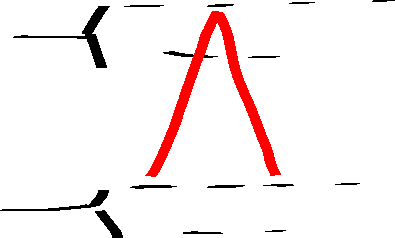
\includegraphics{\imagepath/gray_molasses_level_diagram/gray_molasses_level_diagram.pdf}
    \caption{Level diagram of the D$_1$ line of lithium. The $\Lambda$-system used in gray molasses cooling consists of two manifolds with equal $J$, made up of two magnetic sublevels in the ground state and one in the excited state.}\label{fig:gray_molasses_level_diagram}
\end{figure}

The counter-propagating gray molasses beams have circular polarization. At every point the superposition of the polarizations yields an effective polarization that is sensed by the atoms. This effective polarization depends on the phase of the two light beams with respect of each other, that means that the atoms see alternating circular, elliptical, linear, elliptical, etc. polarization along their journey through the light field. This makes the coupling between the relevant states position-dependent, as shown in figure~\ref{fig:gray_molasses_polarization_gradient}.

\begin{figure}
    \centering
    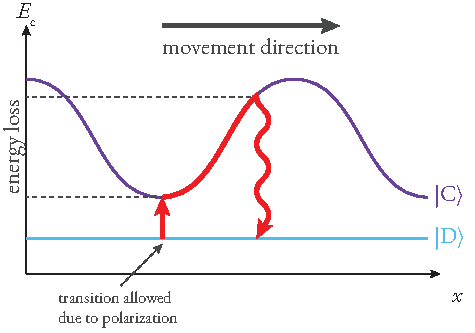
\includegraphics{\imagepath/gray_molasses_polarization_gradient/gray_molasses_polarization_gradient.pdf}
    \caption{Polarization-gradient in the gray molasses scheme: Atoms move along the light field and see different energy shifts depending on their position. At positions with low light shift, they transition from the dark state $\Ket{\text{D}}$ to the coupling state $\Ket{\text{C}}$ and move further losing kinetic energy in the polarization gradient field until they decay back.}\label{fig:gray_molasses_polarization_gradient}
\end{figure}

In the gray molasses' light field, the $\Lambda$-system is dressed with two orthogonal, hence not mutually coupling, eigenstates $\Ket{\text{C}}$ and $\Ket{\text{D}}$, being superpositions of the two ground states. One of them, $\Ket{\text{C}}$, couples to the light field via the excited state and experiences an energy shift $E_C \propto \frac{\Omega_\text{eff}^2}{\delta}$. The other, $\Ket{\text{D}}$, is a dark state~\cite{weidemuller_novel_1994,gerken_gray_2016}.

The absence of coupling between these two states only persists as long as the atoms' kinetic energy is not considered. For atoms with momentum $p$, there is a non-zero transition probability $P \propto \left|\frac{p}{E_C} \right|^2$~\cite{weidemuller_novel_1994}. This means that faster atoms are more prone to transition from the dark state to the coupling state, and that this transition is most likely in areas with low light intensity.

The cooling effect in this scheme can now be understood as follows: Atoms move along the gray molasses light field with a finite velocity $v$. At points with low light intensity, due to the polarization gradient, they are likely to transition from the dark state $\Ket{\text{D}}$ to the coupling state $\Ket{\text{C}}$. Moving further in the polarization-gradient field, their light shift energy $E_C$ increases, at the cost of their kinetic energy. When they spontaneously decay back into the dark state $\Ket{\text{D}}$ they lose an amount of energy on the order of the light shift $E_C$. This is illustrated in figure~\ref{fig:gray_molasses_polarization_gradient}. The gray molasses light needs to be blue detuned, $\delta > 0$, because then the light shift is positive, and the atoms lose energy falling back into the dark state $\Ket{\text{D}}$. With this scheme,  temperatures even below the recoil limit $T_\text{recoil}$ can be reached~\cite{weidemuller_novel_1994,gerken_gray_2016}.


\paragraph{Gray Molasses with Lithium} The D$_1$ line of lithium is just \SI{10}{\giga\hertz} off the D$_2$ line. This avoids the need for separate laser system in a different wavelength regime and  enables reusing optics of the magneto-optical trap for the gray molasses. Similar to the magneto-optical trap, a cooler and a repumper are needed: the former is blue detuned with respect to the $\Ket{^2\text{S}_{1/2}, F = 3/2} \rightarrow \Ket{^2\text{P}_{1/2}, F = 3/2}$ transition, the latter is blue detuned with respect to the $\Ket{^2S_{1/2}, F = 1/2} \rightarrow \Ket{^2\text{P}_{1/2}, F = 3/2}$. In contrast to cooling on the D$_2$ line, the excited manifold of the D$_1$ line is resolved, meaning the splitting between its excited state's hyperfine level is larger than its line width~\cite{gerken_gray_2016}.

\citeauthor{burchianti_efficient_2014} implemented gray molasses for fermionic lithium in 2014. Their parameters were taken as a reference starting point for configuring the gray molasses of the FermiQP demonstrator setup~\cite{burchianti_efficient_2014}:
\begin{itemize}
    \item laser intensities: $s_{0, \text{cooler}} = 2.7$, $\frac{I_\text{repumper}}{I_\text{cooler}} \approx 0.2$
    \item detunings: $\delta_\text{cooler} = +5.4 \Gamma$, varying $\delta_\text{repumper}$ between $(\delta_\text{cooler} -2 \Gamma)$ and  $(\delta_\text{cooler}+ 3\Gamma)$
\end{itemize}
with $I_s = \SI{7.59}{\milli\watt\per\square\centi\meter}$ and $\Gamma = \SI{5.8724}{\mega\hertz}$ for the D$_1$ line~\cite{gehm_properties_2003}.


\section{The 3-dimensional Magneto-optical Trap of the FermiQP Demonstrator}
\todo{Make clear what is done already and what is still outstanding.}
In this section, the geometry, the laser setup, the optics and the magnetic gradients for the 3-dimensional magneto-optical trap in the FermiQP demonstrator will be discussed. Due to massive supply chain problems and delivery time extensions by part vendors, only the laser setup [[and optics]] could be built during the writing of the thesis. For the other aspects of the trap, details of planning and simulations are presented.

\subsection*{Geometry}
The 3-dimensional magneto-optical trap of the FermiQP demonstrator is loaded from the atomic beam originating from the 2-dimensional magneto-optical trap. It is guided through a differential pumping stage separating the high and the ultra-high vacuum regions of the experiment chamber. The trap is located in the front part of the glass cell. The space around the glass cell is tightly packed with the two microscope objectives sitting above and below the trap and the Feshbach coils placed left and right of the incoming atomic beam, as shown in figure~\ref{fig:glass_cell_vicinity}. As a reminder, the reference coordinate system of the experiment chamber is that $x$ is along the atomic beam, $y$ is to the left as seen in the direction of the atomic beam, and $z$ is in upward direction.

\begin{figure}
    \centering
    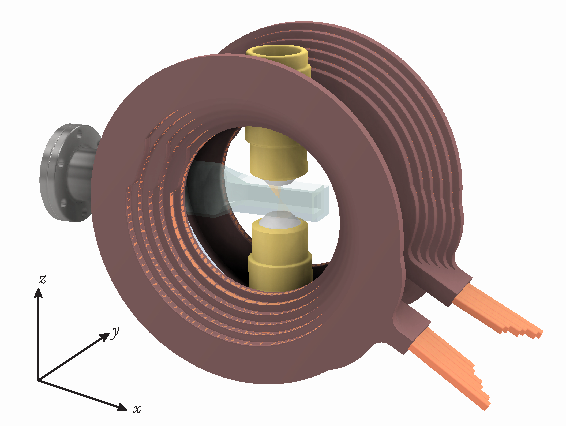
\includegraphics{\imagepath/glass_cell_vicinity/glass_cell_vicinity.pdf}
    \caption{Position of the glass cell between the microscope objectives and the Feshbach coils. The tightly packed vicinity of the glass cell determines the geometry of the magneto-optical trap.}\label{fig:glass_cell_vicinity}
\end{figure}

The magneto-optical trap needs three pairs of beams, one for each spatial degree of freedom that the atoms should be cooled along. For each pair, a beam is shot in from one side and retroreflected after passing through the glass cell. Due to the tightly packed vicinity of the glass cell, the beam axes cannot match with the Cartesian coordinate axes: no beams can be shot along the $z$ axis which is blocked by the objectives, and no beam can be shot directly along the atomic beam axis ($x$) because no retroreflection would be possible on the other side of the glass cell.

Instead, two beams are shone in in the $xz$ plane at an angle with respect to the atomic beam. The geometry of the microscope objectives only permits shooting beams into the glass cell at shallow angles, namely with an incidence angle of \SI{60}{\degree} with respect to the surface normal of the glass cell, as depicted in figure~\ref{fig:glass_cell_sides_mot_beams_0}. These beams provide cooling and confinement along the atomic beam axis ($x$, with an angle $\theta = \SI{30}{\degree}$ between light propagation $\vec k$ and velocity $\vec v$ of the atomic beam) and the up-down axis ($y$). The third beam is shot in along the $y$ axis, i.e.\ from left to right (see figure~\ref{fig:glass_cell_sides_mot_beams_1}). The beams are reflected back on reflection stages behind the glass cell.

\begin{figure}
    \centering
    \begin{subfigure}{0.49\textwidth}
        \centering
        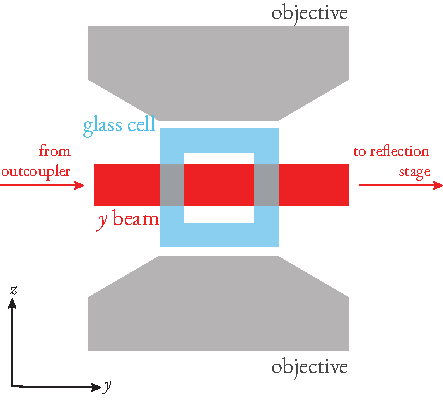
\includegraphics[scale=0.45]{\imagepath/glass_cell_sides_mot_beams/glass_cell_sides_mot_beams_0.pdf}
        \caption{View perpendicular to the atomic beam [[add objective]]}\label{fig:glass_cell_sides_mot_beams_0}
    \end{subfigure}
    \begin{subfigure}{0.49\textwidth}
        \centering
        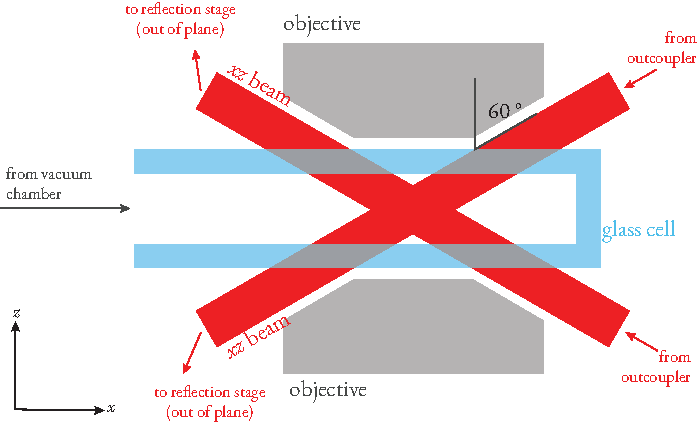
\includegraphics[scale=0.45]{\imagepath/glass_cell_sides_mot_beams/glass_cell_sides_mot_beams_1.pdf}
        \caption{View against the atomic beam [[add objective]]}\label{fig:glass_cell_sides_mot_beams_1}
    \end{subfigure}
    \caption{Schematic side views of the glass cell: The two magneto-optical trap beams on the axis of the atomic beam come in under shallow angles of \SI{30}{\degree}.
    \todo[inline]{hint to reflection stage position, show vacuum chamber position, add angles}
    }\label{fig:glass_cell_sides_mot_beams}
\end{figure} 

\subsection*{Cooling Laser Setup}
The cooling laser beams for the 2-dimensional and the 3-dimensional magneto-optical traps as well as for the gray molasses are jointly produced on an optics board from where they are transferred to the experiment chamber via optical fibers.

The laser beams originate from two laser sources, one for D$_2$ light for the magneto-optical traps and one for D$_1$ light for the gray molasses. All beams produced by the setup consist of cooler and repumper light, which is separated by \SI{228}{\mega\hertz}, the hyperfine splitting of the $^2\text{S}_{1/2}$ ground state. For the 2-dimensional magneto-optical trap, the frequencies of the cooler and repumper light as well as their powers are fixed, for the 3-dimensional trap and the gray molasses light they need to be variable in order to compress and optimize the traps dynamically. The light for the 3-dimensional trap and the gray molasses cooling should be prepared on the same optical path, which is useful as both cooling schemes are carried out at the same position in the experiment chamber. All beams need to have sufficient power levels such that several saturation intensities on the respective trap cross-sections (\SI{30}{\milli\meter} for the 2-dimensional trap and \SI{7}{\milli\meter} for the 3-dimensional trap and the gray molasses cooling).

\paragraph{Laser sources}
The \SI{671}{\nano\meter} laser light for the D$_2$ and D$_1$ lines is jointly produced for all aforementioned cooling beams by two Raman fiber amplifiers (MPB VRFA-P-1500-671-SF-PLUS, "Socrates" and "Plato") with a specified output power of \SI{1.5}{\watt} each. They are supplied with seed light by two single-mode diode lasers at \SI{1342}{\nano\meter} (Toptica MDL pro, "Heraklitus" seeding "Socrates", and "Zeno" seeding "Plato"), delivering around \SI{20}{\milli\watt} of power. Each fiber amplifier contains a frequency-doubling stage creating \SI{671}{\nano\meter} light from the amplified \SI{1342}{\nano\meter} light. The seed lasers are offset-locked to a global reference laser that itself is locked to an ultra-low expansion cavity. The offset locking allows shifting the laser frequencies of the D$_2$ and the D$_1$ light arbitrarily within a range of a few hundred \si{\mega\hertz} \todo{verify}. The interplay of these lasers is outlined in figure~\ref{fig:laser_interplay_schematic}.

\begin{figure}
    \caption{Schematic of the cooling laser setup: Two Raman fiber amplifiers provide light for the optics setups that prepare the light used in the magneto-optical traps and the gray molasses. The amplifiers are offset-locked via their seeds to a global reference lasers which, in turn, is locked to a reference cavity.}\label{fig:laser_interplay_schematic}
\end{figure}


The main advantage of using the Raman fiber amplifiers is that they produce enough optical power to simultaneously supply all three aforementioned traps with light. An alternative would be separate laser sources, each of which would need to be frequency-locked and monitored independently. During the writing of the thesis, the Raman fiber amplifiers showed signs of substantial degradation as their output power decreased by over \SI{20}{\percent} in only a few weeks of intermittent operation. The details and the severity of this degradation are presented in~\cite{qesja_design_2022}. As the experimenters of FermiQP, as well as the manufacturers, could not come up with a quick and reliable solution to this problem, it stays uncertain whether the Raman fiber amplifiers can be used long-term for the laser cooling within the FermiQP demonstrator. An alternative approach would be amplification of the seed light using tapered amplifier chips.


\paragraph{Outline of the Laser Setup}
The necessary output beams for the traps and the gray molasses are created from the two input beams on the D$_2$ and the D$_1$ frequency as depicted in figure~\ref{fig:laser_setup_schematic}.

\begin{figure}
    \centering
    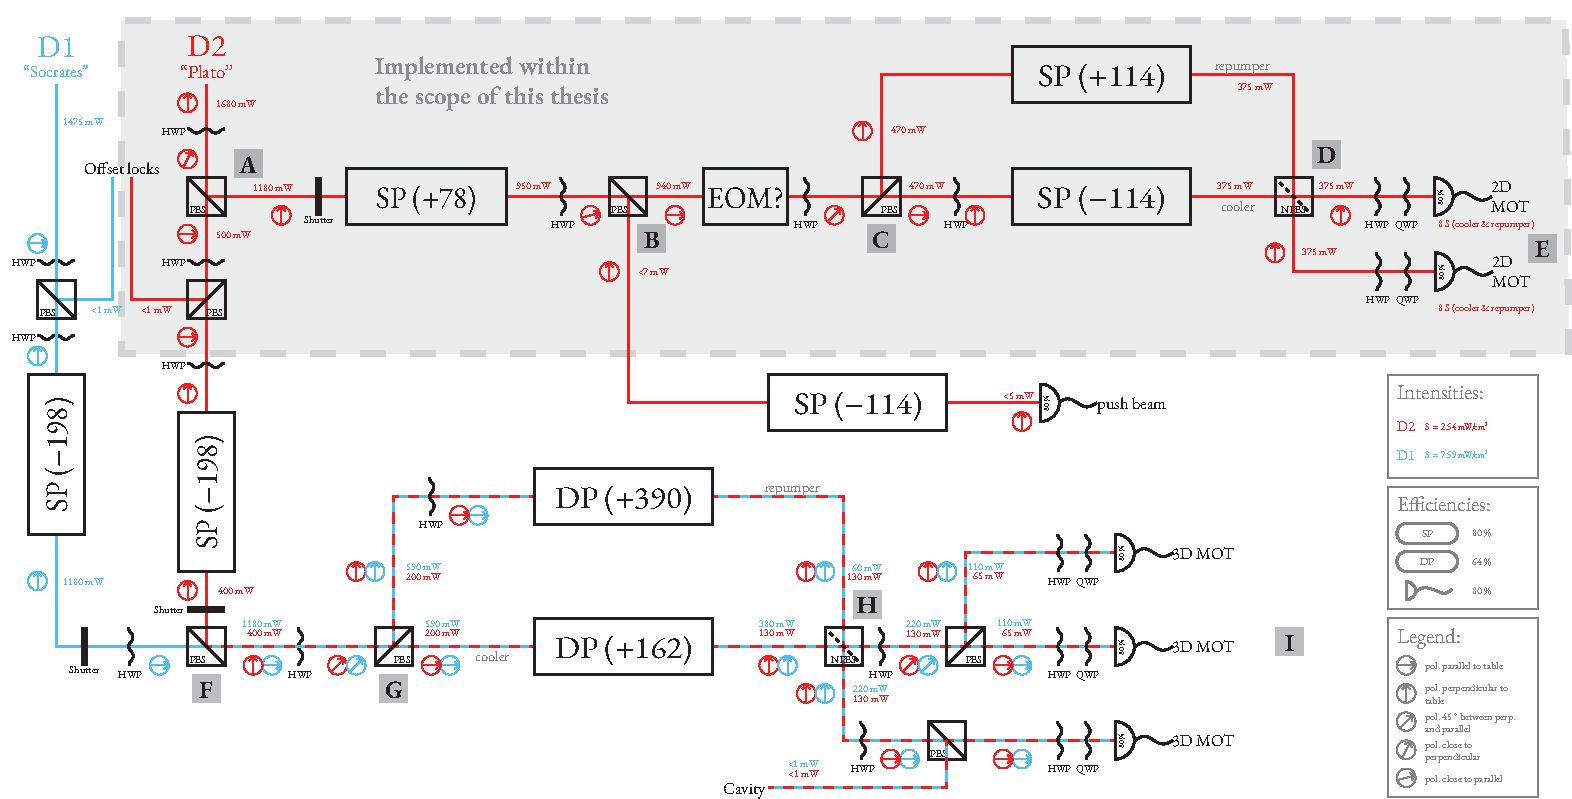
\includegraphics[width=\textwidth]{\imagepath/laser_setup_schematic/laser_setup_schematic.pdf}
    \caption{Schematic of the laser setup for preparing the cooling light for the magneto-optical traps and the gray molasses: D$_2$ light is split into two branches for the 2-dimensional (to the right) and the 3-dimensional magneto-optical (to the bottom) traps at the first PBS (A).
    For the light for the 2-dimensional trap, a small amount of power is taken out for the push beam (B) before it is split into cooler and repumper (C) light for the two outputs. It is considered to add an electro-optical modulator for improving the cooling effect of the light. This part of the laser setup was constructed within the scope of this thesis.
    The light for the 3-dimensional trap and the D$_1$ light for the gray molasses are spatially overlapped (D), split into cooler and repumper (E), and then distributed into three outputs (F).
    (Abbreviations: SP and DP boxes stand for single pass and double pass acousto-optical modulators respectively, the number denotes the applied frequency in \si{\mega\hertz}. PBS stands for polarizing beam splitter. HWP and QWP stand for half and quarter wave plate.)
    \todo[inline]{TODO update image: remove unnecessary details, remove powers, add 2D-MOT board boundary, adapt font, adapt colors, add letter markers, add RFA names, add EOM}}
    \label{fig:laser_setup_schematic}
\end{figure}

The D$_2$ light is offset-locked \SI{-78}{\mega\hertz} below the actual D$_2$ transition frequency. It is split into on a polarizing beam splitter into a path for the 2-dimensional and one for the 3-dimensional magneto-optical trap. The power splitting ratio can be adjusted using a half-wave plate and was preliminarily set to about $\frac{1}{3}$ for the 3-dimensional and $\frac{2}{3}$ for the 2-dimensional optical trap since the 2-dimensional trap needs to reach the required intensity for a larger trap cross-section, and it is the first cooling stage of the experiment bridging the large range from several hundred Kelvin to sub-Kelvin temperatures on two of three spatial axes.

The branch for the 2-dimensional trap can be blocked using a shutter and an acousto-optical modulator. The modulator deflects a beam on its main order depending on its radio-frequency input power. By blocking the path of non-deflected beams after it and letting through the path of deflected beams, it can be used as a fast optical switch steered by the experiment control system. The shutter is a loudspeaker magnet with a beam blocker attached to it and acts as an additional slow controllable beam blockade ensuring that definitely no light can pass. This acousto-optical modulator increases the laser frequency by \SI{+78}{\mega\hertz} such that the light is resonant with the D$_2$ transition again. Using another half-wave plate and beam splitter, a small fraction of the laser power is branched off for the push beam. This light is frequency-shifted by \SI{+114}{\mega\hertz} in order to be resonant with the cooler transition. The remaining light is used in the trap. The experimenters consider adding an electro-optical modulator at this point for improving the trap. This modulator would add frequency sidebands at \si{\mega\hertz} to the light. In the trap, these additional frequencies would address other velocity classes than the original light and might hence increase the loading rate of the trap.
After that the light is split in a power ratio of approximately $1$:$1$ into cooler and repumper beams, each of which is fed through an acousto-optical modulator with driving frequencies of \SI{-114}{\mega\hertz} and \SI{+114}{\mega\hertz} for cooler and repumper respectively, which corresponds to the hyperfine splitting of the ground state manifold. Afterwards these two beams are spatially overlapped on a beam splitter and fed to two optical fibers leading to the experiment chamber.

From the branch of the D$_2$ light for the 3-dimensional trap, a small amount is branched off for offset-locking. The remaining light is sent through a modulator-shutter combination for programmatic beam blocking as explained above, here with a modulator frequency of \SI{-198}{\mega\hertz}. It is then spatially overlapped with the D$_1$ light. The D$_1$ light is also offset by \SI{+78}{\mega\hertz}, a part of it split off for offset locking, and fed through an identical programmatic beam blockade. The combined beam of D$_2$ and D$_1$ light is then also split into two paths for cooler and repumper in a ratio of approximately $1$:$1$. Here, however, the light is fed through acousto-optical modulator double-passes as described in~\cite{qesja_design_2022}. In these double-passes the light crosses the modulators twice in an arrangement of a quarter-wave plate, a mirror, and a polarizing beam splitter. As the net deflection is zero in this configuration, it allows a programmatic change of the frequency shift applied to each beam without the need to realign optical components. Together with the ability to damp the laser power by reducing the modulators' radio-frequency driving power, frequency and power of each beam can be independently steered for compressing the 3-dimensional magneto-optical trap and for switching the powers when applying the gray molasses. The cooler beam is frequency shifted by about \SI{+162}{\mega\hertz}, the repumper by about \SI{+390}{\mega\hertz}, with the double-passes allowing for an adjustment range of several tens of \si{\mega\hertz}. The total frequency shift considering the initial offset, the blockade modulators and modulator in the cooler (repumper) path amounts to $\SI{-78}{\mega\hertz} - \SI{198}{\mega\hertz} + \SI{390}{\mega\hertz} = \SI{+114}{\mega\hertz}$ ($\SI{-78}{\mega\hertz} - \SI{198}{\mega\hertz} + \SI{162}{\mega\hertz} = \SI{-114}{\mega\hertz}$) which is again the hyperfine splitting of the ground state manifold.

\paragraph{Implementation of the Laser Setup for the 2-dimensional Magneto-optical Trap}
Within this thesis, the part of the laser setup providing the light for the 2-dimensional magneto-optical trap, as highlighted in figure~\ref{fig:laser_setup_schematic}, was built. The implementation is described in greater detail in this paragraph, figure~\ref{fig:2d_mot_setup_photo} shows a photograph of this part of the setup. For each step, the corresponding marking from the figure is given for orientation.

\begin{figure}
    \centering
    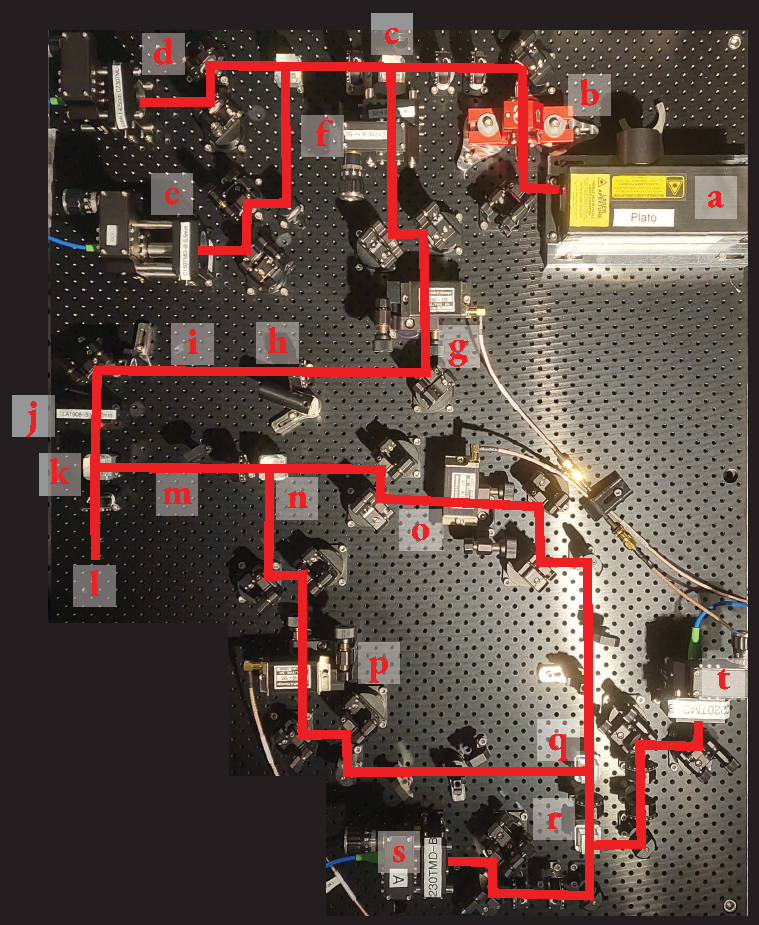
\includegraphics[width=\textwidth]{\imagepath/2d_mot_setup_photo/2d_mot_setup_photo.pdf}
    \caption{Photograph of the part of the optics setup providing light for the 2-dimensional magneto-optical trap. The beam path and reference points from figure~\ref{fig:laser_setup_schematic} have been added for orientation.}\label{fig:2d_mot_setup_photo}
\end{figure}

\begin{itemize}
    \item[a] The D$_2$ light is coming from the doubling stage of the Raman fiber amplifier "Plato" where the amplified \SI{1342}{\nano\meter} light is frequency-doubled to \SI{671}{\nano\meter} light. At this point, the laser beam has an $\frac{1}{\text{e}^2}$ diameter of about \SI{1000}{\micro\meter}.

    \item[b] In order to prevent any inadvertent reflections travelling back into the amplifier, a Newport optical isolator (Newport ISO-04-650-MP-WP) was placed immediately after the doubling stage. In a power measurement, \SI{30}{\deci\bel} damping (with the isolator inverted) and \SI{95}{\percent} transmission could be attested in agreement with the specifications.

    \item[c] After the optical isolator, a quarter-wave plate is used to eliminate any elliptical polarization components from the beam caused by hitting mirrors with light that has polarization other than $\Ket{\text{H}}$ and $\Ket{\text{V}}$.

    \item[d] The D$_2$ light is split into the paths for the different magneto-optical traps with a half-wave plate and a polarizing beam splitter from CeNing optics ([[part number]]) with a specified transmission extinction ratio error of $\frac{1}{1000}$. All other polarizing beam splitters in the same setup are of the same model and specifications. The splitting ratio between the beams was not yet fixed during the course of this thesis.

    \item[e, f] The light transmitted on this beam splitter is again split and coupled into optical fibers leading to the offset lock (f) and to the other optics board hosting the rest of the setup (e, for details see~\cite{qesja_design_2022}). The light reflected off on the beam splitter is used for the push beam and the 2-dimensional magneto-optical trap.

    \item[g] As the acousto-optical modulators used in the setup require way smaller beam diameters than the \SI{1000}{\micro\meter} beam output by the Raman fiber amplifier, a telescope for decreasing the beam diameter was placed after the aforementioned beam splitter cube. The telescope consists of a convex lens ($f = \SI{75}{\milli\meter}$) focusing the beam and a concave lens ($f = \SI{-50}{\milli\meter}$) after about \SI{30}{\milli\meter}. This reduces the beam diameter to about \SI{650}{\micro\meter} immediately after the second lens, the beam waist is now about $2w_0 = \SI{600}{\micro\meter}$ located about \SI{175}{\milli\meter} away from the telescope. Lowering the beam diameter is a trade-off between a slimmer beam waist $w_0$ making the beam fitting better into the acousto-optical modulators' apertures and a larger beam divergence $\theta = \frac{\lambda}{\pi w_0}$ that would lead to even larger beam diameters after some propagation distance. The scaled-down beam reaches a diameter of about \SI{700}{\micro\meter} after about \SI{475}{\milli\meter} after the telescope. In order to scale it down for the rest of the beam path on the board, a convex lens ($f = \SI{500}{\milli\meter}$) was placed in the beam path. In this way, the beam diameter is kept under \SI{700}{\micro\meter} on the remaining beam path with the waist (diameter $2w_0 \approx \SI{650}{\micro\meter}$) at a total distance of \SI{720}{\milli\meter} from the telescope.  These parameters were estimated based on a simulation in the software GaussianBeam\footnote{\url{https://sourceforge.net/projects/gaussianbeam/}}, shown in figure~\ref{fig:beam_diameter_evolution}.

\begin{figure}
    \caption{Evolution of the beam shape from the telescope along the beam path}
    \label{fig:beam_diameter_evolution}
\end{figure}

    \item[h] The slimmed-down light is then coupled through the first acousto-optical modulator (Gooch \& Housego 3080-120, \SI{80(10)}{\mega\hertz}, aperture \SI{1}{\milli\meter}). This modulator is operated at \SI{+78}{\mega\hertz}. The zeroth order of the outgoing beam is blocked at i. The power efficiency of this acousto-optical modulator single pass is \todo{add AOM efficiency}. Thanks to the telescope, the beam diameter at this point is significantly smaller than the specified aperture.
    
    \item[i] A half-wave plate sets the splitting ratio between light for the push beam (m) and light for the 2-dimensional magneto-optical trap.
    
    \item[j] At this position the shutter will be placed in order to be able to completely bar any light from entering the magneto-optical trap.
    
    \item[k] Here the light is refocused using an $f = \SI{500}{\milli\meter}$ lens as described for point g. This sizes down the beam diameter such that it doesn't exceed the aperture of the acousto-optical modulators for creating the cooler and repumper beams (p, q).
    
    \item[l] The light is split into a few \si{\milli\watt} for the push beam (m) and the rest for the 2-dimensional magneto-optical trap.

    \item[m] Here the push beam light will be prepared using single pass acousto-optical modulator driven at \SI{+114}{\mega\hertz} which serves as a frequency shifter and as a shutter.
    
    \item[n] At this point, space is left free for an electro-optical modulator that would add sidebands onto the light allowing for addressing more velocity classes in the trap and thus increasing its loading rate.
    
    \item[o] With a half-wave plate and a polarizing beam splitter, the light is split into cooler (q) and repumper (p) paths. The polarizations of the beams are $\KetText{V}$ of the cooler and $\KetText{H}$ of the repumper beam.
    
    \item[p, q] The cooler (q) and repumper  (p) paths contain acousto-optical modulators (Gooch \& Housego 3110-120, \SI{110(12)}{\mega\hertz}, aperture \SI{0.6}{\milli\meter}). Thanks to the refocusing lens (k), the beam diameter approximately matches the modulators' apertures. The power efficienies are \todo{add AOM efficiencies} for the cooler and for the repumper.
    
    \item[r, s] The cooler and repumper beam are spatially overlapped in split into two paths on a combination of two polarizing beam splitter cubes and a half-wave plate. Due to their polarizations, the cooler is reflected on the first cube (r) while the repumper passes through it, both leaving the cube on the same port. A half-wave plate then turns their respective polarizations to diagonal $\KetText{D}$ and anti-diagonal $\KetText{A}$. A subsequent polarizing beam splitter cube (s) splits both cooler and repumper into two equally strong beams.
    
    \item[t, u] The two resulting beams are coupled into fibers guiding it to the experiment chamber. In each beam, a pair of a quarter- and half-wave plate allow for arbitrary corrections of the polarization if necessary. The coupling efficiencies are \todo{add coupling efficiences}.
\end{itemize}

Table \ref{tab:power_cascade} outlines how much power is dissipated on the optics board and gives exemplary numbers for a typical mode of operation.

\begin{table}
    \begin{tabularx}{\textwidth}{ccc}
        \toprule
        after board element & relative power & exemplary power \\
        \midrule
        a & \SI{100}{\percent} & \SI{1500}{\milli\watt}\\
        b && \\
        ... && \\
        \bottomrule
    \end{tabularx}
    \caption{Power dissipation on the board creating the light for the 2-dimensional magneto-optical trap.
    \todo[inline]{Fill in power levels}
    }
    \label{tab:power_cascade}
\end{table}


\subsection*{Optics around the Experiment Chamber}
The six cooling laser beams for the 3-dimensional magneto-optical trap are transferred from the optics board to the experiment chamber with optical fibers. 

One trap beam will be shot in from the left or right side of glass cell and will be reflected back directly on a reflection stage at the other side of the glass cell. The two other beams are shot into the glass cell from the upper and lower front of the glass cell through the upper sides at an angle of \SI{60}{\degree} with respect to glass surface in order not to be blocked by the microscope objectives (as explained in the geometry section above, see figure~\ref{fig:glass_cell_sides_mot_beams}). For reflecting these beams back into the glass cell, they are first guided away from the experiment chamber onto stand-alone reflection stages as there wouldn't be enough space for these stages between the experiment chamber and the glass cell (see figure~\ref{fig:mot_optics_schematic_from_above}).

\begin{figure}
    \caption{Schematic of the optics for the 3-dimensional magneto-optical trap from above}
    \label{fig:mot_optics_schematic_from_above}
\end{figure}

\paragraph{Optics Stages}
The outcoupling stages consist of optical elements for collimating, polarization-cleaning, and polarization-preparing the light, mounted in an optical cage system. A schematic of the stage is shown in figure~\ref{fig:outcoupling_stage_schematic}

\begin{figure}
    \centering
    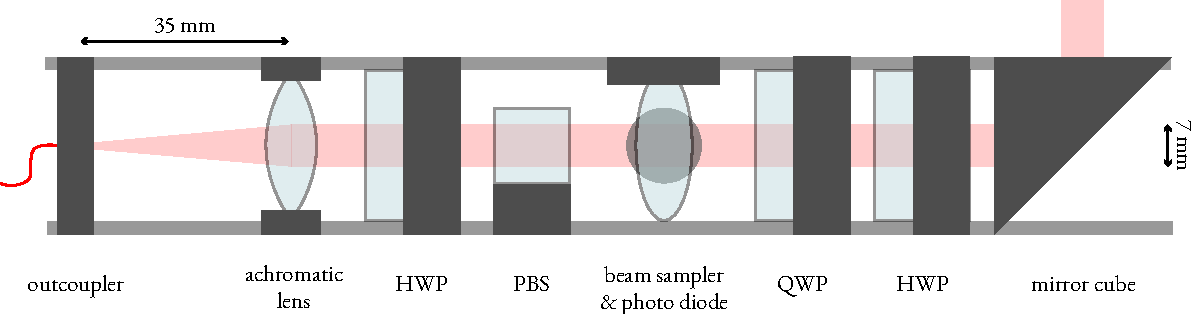
\includegraphics[width=\textwidth]{\imagepath/outcoupling_stage_schematic/outcoupling_stage_schematic.pdf}
    \caption{Schematic of the outcoupling stage in an optical cage system: The trapping light coming from an optical fiber is collimated with an achromatic lens such that the beam has a $\frac{1}{e^2}$ diameter of \SI{7}{\milli\meter}. The polarization is cleaned using a half-wave plate and a polarizations beam splitter. Using a beam sampler, a small amount of light is reflected out of the axis and shot onto a photodiode for power monitoring. The light is polarization-prepared on a quarter- and a half-wave plate.}
    \label{fig:outcoupling_stage_schematic}
\end{figure}

The light leaving the optical fiber has a divergence angle of $\theta = \frac{\lambda}{\pi w} = \frac{\SI{671}{\nano\meter}}{\pi\SI{2.25}{\micro\meter}} = \SI{95}{\milli\radian}$ with the beam waist $w = \SI{2.25}{\micro\meter}$ at the fiber tip. In order to collimate it to a beam of $\frac{1}{e^2}$ diameter of \SI{7}{\milli\meter}, hence radius of $r_{1/e^2} = \SI{3.5}{\milli\meter}$, a lens of focal length $f = \frac{r_{1/e^2}}{\tan \theta} = \frac{\SI{3.5}{\milli\meter}}{\SI{95}{\milli\radian}} \approx \SI{35}{\milli\meter}$~\cite{noauthor_collimated_2021} is installed in the outcoupling stage such that the fiber tip is in the focal point.

In order to clean the polarization that the light might have acquired while travelling in the fiber, is cleaned using a combination of a half-wave plate and a polarizing beam splitter.

After that a beam sampler reflects out a small fraction of the light onto a photodiode for power monitoring. Note that the power is monitored after polarization cleaning in order to check the effective power that is available for trapping\footnote{The power is not monitored on the other beam splitter port as then one could not distinguish between polarization-induced and supply-induced power changes. It is also not checked by monitoring the transmitted power on one of the system's mirrors as the absolute power transmitted through these mirrors would be too little.}.

Finally, the polarization of the trapping beam can be set using a quarter- and a half-wave plate.

The reflection stages consist of a quarter- and a half-wave plate and a mirror mounted in a cage system, as depicted in figure~\ref{fig:reflection_stage_schematic}.

\begin{figure}
    \centering
    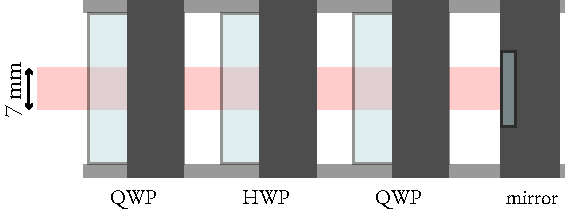
\includegraphics[scale=0.77]{\imagepath/reflection_stage_schematic/reflection_stage_schematic.pdf}
    \caption{Schematic of the reflection stage in an optical cage system: Incoming light is sent through a quarter- and a half-wave plate, reflected on a mirror, and leaves the stage propagating through the two wave plates again in reverse order.}
    \label{fig:reflection_stage_schematic}
\end{figure}

\paragraph{Polarization}
The trapping light needs to have circular polarization at the trap position in the glass cell, either with left or right helicity for both the forward and the backward pass, depending on the direction of the magnetic gradient. Since the polarization cannot be measured within the glass cell at the time of operation, the approximate configuration of the optics for attaining the necessary polarization was estimated.

In the following, the Jones vector notation for polarization in the $\{\KetText{H}, \KetText{V}\}$ basis is going to be used to denote circular and diagonal polarization:
\begin{align}
        \KetText{R} &= \frac{1}{\sqrt{2}} \left(\KetText{H} - i \KetText{V}\right)  & \KetText{L} &= \frac{1}{\sqrt{2}} \left(\KetText{H} + i \KetText{V}\right) \\
        \KetText{D} &= \frac{1}{\sqrt{2}} \left(\KetText{H} + \KetText{V}\right)  &  \KetText{A} &= \frac{1}{\sqrt{2}} \left(\KetText{H} - \KetText{V}\right)
\end{align}

For the trap beam entering the glass cell from the left or right, the circular polarization can directly be set on the wave plates in the outcoupling stage. As the light enters the glass cell perpendicular to its surface, the polarization will stay unchanged when transmitted through the glass.

For the other two beams entering at shallow angles with $\theta = \SI{60}{\degree}$ between the surface normal and the beam, the different values of the transmission coefficients for $\KetText{H}$ and $\KetText{V}$ polarization components need to be considered and the wave plates on the outcoupling and the reflection stages must be set accordingly.

The glass cell is made of fused silica with a refractive index of $n = \SI{1.456}{}$ at \SI{671}{\nano\meter} \cite{malitson_interspecimen_1965}. According to Snell's law, the angle between the light and the surface normal in the glass is $\theta_\text{glass} = \arcsin \frac{\sin \theta}{n} = \SI{36.5}{\degree}$~\cite{demtroder_elektromagnetische_2013}. The transmission coefficients for the polarization components are~\cite{demtroder_elektromagnetische_2013}
\begin{align}
    \begin{split}
        t_{\KetText{H}, \text{air} \rightarrow \text{glass}} &= \frac{2 \cos \theta}{\cos \theta + n \cos \theta_\text{glass}} =  \SI{0.916}{}\\
        t_{\KetText{H}, \text{glass} \rightarrow \text{air}} &= \frac{2n \cos \theta_\text{glass}}{n \cos \theta_\text{galss} + \cos \theta} = \SI{0.999}{} \\
        t_{\KetText{V}, \text{air} \rightarrow \text{glass}} &= \frac{2 \cos \theta}{n \cos \theta + \cos \theta_\text{glass}} = \SI{0.916}{}\\ 
        t_{\KetText{V}, \text{glass} \rightarrow \text{air}} &= \frac{2 n \cos \theta_\text{glass}}{\cos \theta_\text{glass} + \cos \theta} = \SI{0.999}{}\\ 
    \end{split}
\end{align}
\begin{align}
    \begin{split}
        t_{\KetText{H}} = t_{\KetText{H}, \text{air} \rightarrow \text{glass}}  \cdot t_{\KetText{H}, \text{glass} \rightarrow \text{air}} = \SI{0.839}{} \\
        t_{\KetText{V}} = t_{\KetText{V}, \text{air} \rightarrow \text{glass}}  \cdot t_{\KetText{V}, \text{glass} \rightarrow \text{air}} = \SI{0.998}{}
    \end{split}
\end{align}
\todo{check}
where the $\text{s}$ and $\text{p}$ components of the polarization have been identified with the $\KetText{H}$ and $\KetText{V}$ basis vectors respectively.


In order to attain circular polarization on the first pass through the glass cell, these polarization-dependent losses need to be pre-compensated when choosing the polarization before the glass cell surface:
\begin{align}
    \label{eq:predicted_polarization_first_pass_right}
    \text{for right polarization:} \hspace{1cm} & \frac{\KetText{H}}{t_{\KetText{H}}} - i \frac{\KetText{V}}{t_{\KetText{V}}} \propto 0.765 \KetText{H} - 0.644i \KetText{V} \\
    \label{eq:predicted_polarization_first_pass_left}
    \text{for left polarization:} \hspace{1cm} & \frac{\KetText{H}}{t_{\KetText{H}}} + i \frac{\KetText{V}}{t_{\KetText{V}}} \propto 0.765 \KetText{H} + 0.644i \KetText{V}
\end{align}

\begin{figure}
    \centering
    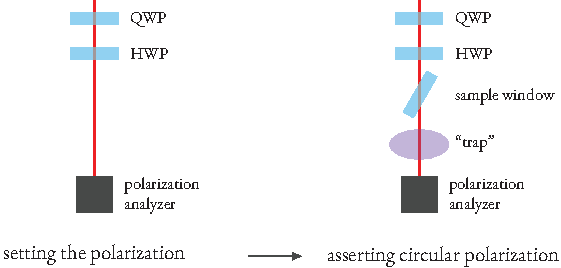
\includegraphics[]{\imagepath/first_pass_polarization_measurement_scheme/first_pass_polarization_measurement_scheme.pdf}
    \caption{Schematic of the experimental setup for verifying the polarization of the incident trapping light for the first pass through the glass cell: At first, the predicted polarizations (equations~\eqref{eq:predicted_polarization_first_pass_right} and~\eqref{eq:predicted_polarization_first_pass_left}) were set and verified using a polarization analyzer. Then a sample glass plate was put in and circular polarization after the plate (the ``trap'' position) was asserted.}
    \label{fig:first_pass_polarization_measurement_scheme}
\end{figure}

For verifying these polarization presets in a mock setup, a sample fused silica glass plate of thickness \SI{4.04}{\milli\meter} was placed at an angle of \SI{60}{\degree} with respect to a \SI{671}{\nano\meter} laser beam. This glass plate acts as the surface which the light enters the glass cell through. Using a pair of a quarter- and a half-wave plate, the polarization before the plate could be arbitrarily set by monitoring it on a polarization analyzer. Then the glass plate was put into the beam path and and circular polarization was asserted after the glass plate, as outlined in figure~\ref{fig:first_pass_polarization_measurement_scheme}. The results are displayed in table~\ref{tab:polarization_first_pass} and show that the aforementioned estimated polarizations  are a good estimate for producing circular polarization in the glass cell.

\begin{table}
    \begin{tabularx}{\textwidth}{ccc}
        \toprule
        target polarization & set before glass plate & measured after glass plate \\
        \midrule
        $\KetText{R}$ & $0.78 \KetText{H} + (-0.02-0.63i) \KetText{V}$ & $0.70 \KetText{H} +(0.00-0.71i)\KetText{V}$ \\
        $\KetText{L}$ & $0.75 \KetText{H} + (-0.01+0.67i)\KetText{V}$ & $0.70 \KetText{H} + (0.00+0.71i)\KetText{V}$ \\
        \bottomrule
    \end{tabularx}
    \caption{Results of the experimental verification of the preset polarization for the first pass through the glass cell, as outlined in figure~\ref{fig:first_pass_polarization_measurement_scheme}. The measured polarizations after the glass plate confirm that the proposed precompensation (equations~\eqref{eq:predicted_polarization_first_pass_right} and~\eqref{eq:predicted_polarization_first_pass_left}) is a good estimate. All values are outputs of the polarzation analyzer, transformed from the azimuth-ellpticity basis to the Jones basis using the Python library py-pol~\cite{noauthor_python_nodate}. Note that py-pol defines $\KetText{R} = \frac{1}{\sqrt{2}}(\KetText{H}+i\KetText{V}), \KetText{L} = \frac{1}{\sqrt{2}}(\KetText{H}-i\KetText{V})$.}
    \label{tab:polarization_first_pass}
\end{table}

\pagebreak
\todo{check if pagebreak necessary}
In order to attain the same circular polarization on the second pass through the glass cell, the wave plates on the reflection stages must be set accordingly. Their required configuration is determined experimentally since the glass surfaces and mirrors in the beam path introduce many polarization changes that are hard to deduct from principle. Again, a mock setup with a sample glass plate with a shallow angle with respect to the beam is used. Light is transmitted through a polarizing beam splitter cube, circularly polarized using a quarter-wave plate, and then transmitted through the sample glass plate. This time, it acts as the surface which the light leaves the glass cell through. Afterwards the light is deflected through two waveplates onto a mirror which represents the reflection stage. The mirror is adjusted such that the beam passes back through the setup until it reaches the beam splitter cube again. This arrangement is outlined in figure~\ref{fig:second_pass_waveplate_adjustment_scheme}. The ideal wave plate configuration on the reflection stage is now identified by monitoring the power reflected on the polarizing beam splitter depending on the wave plate configuration: For circular light on the backward pass after the glass plate (meaning at the trap position in the mock setup), all light is deflected on the beam splitter cube after passing back through the waveplate. This cascade of polarizations is outlined in~\eqref{eq:second_pass_waveplate_adjustment_cascade_r} and~\eqref{eq:second_pass_waveplate_adjustment_cascade_l}:
\begin{align}
    \label{eq:second_pass_waveplate_adjustment_cascade_r}
    \text{port 1} \underset{\text{beam splitter}}{\longrightarrow} \KetText{H} \underset{\text{QWP}}{\longrightarrow} \KetText{R} \underset{\text{X}}{\longrightarrow} \Ket{\psi_\text{R}}
    & ~~ \underset{\text{mirror}}{\longrightarrow} ~~
    \Ket{\psi_\text{R}}  \underset{\text{X}}{\longrightarrow} \KetText{R} \underset{\text{QWP}}{\longrightarrow} \KetText{V} \underset{\text{beam splitter}}{\longrightarrow} \text{port 2}
    \\
    \label{eq:second_pass_waveplate_adjustment_cascade_l}
    \underbrace{
        \text{port 1} \underset{\text{beam splitter}}{\longrightarrow} \KetText{H} \underset{\text{QWP}}{\longrightarrow} \KetText{L} \underset{\text{X}}{\longrightarrow} \Ket{\psi_\text{L}}
    }_{\text{forward pass}}
    & ~~ \underset{\text{mirror}}{\longrightarrow} ~~ 
    \underbrace{
        \Ket{\psi_\text{L}}  \underset{\text{X}}{\longrightarrow} \KetText{L} \underset{\text{QWP}}{\longrightarrow} \KetText{V} \underset{\text{beam splitter}}{\longrightarrow} \text{port 2}
     }_{\text{backward pass}}
\end{align}
with $\text{X}$ denoting the transmission through the glass plate, deflection on the mirror and through the wave plates on the reflection stage to be adjusted. The polarizations $\Ket{\psi_\text{R}}$ and $\Ket{\psi_\text{L}}$ identify the ideal wave plate configuration and are hence the parameter looked for in the mock setup. $\Ket{\psi_\text{R}}$ and $\Ket{\psi_\text{L}}$ can now be measured by replacing the mirror with the polarization analyzer, as outlined in figure~\ref{fig:second_pass_waveplate_adjustment_scheme}. The identified ideal polarizations are listed in table~\ref{tab:polarization_second_pass}.

\begin{figure}
    \centering
    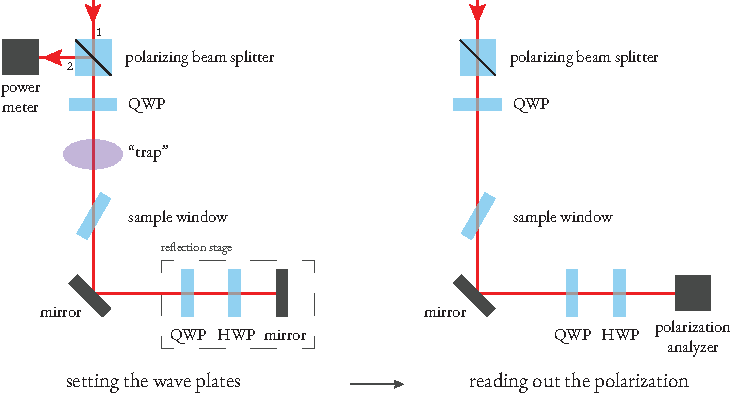
\includegraphics[]{\imagepath/second_pass_waveplate_adjustment_scheme/second_pass_waveplate_adjustment_scheme.pdf}
    \caption{Schematic of the experimental setup for finding the right configuration of the wave plates on the reflection stages: In a first step, the wave plate configuration on the "reflection stage" is optimized for circular polarization in the ``trap'' by maximizing the output power on port 2 of the beam splitter cube. Then the polarization in the reflection stage which identifies the optimal waveplate configuration is measured using a polarization analyzer.}\label{fig:second_pass_waveplate_adjustment_scheme}
\end{figure}

\begin{table}
    \begin{tabularx}{\textwidth}{cl}
        \toprule
        target polarization $P$ & polarization $\Ket{\psi_P}$ in reflection stage \\
        \toprule
        \multirow{4}{*}{$\KetText{R}$} & pol0 \\
        & pol1 \\
        & pol2 \\
        & pol3 \\
        \midrule
        \multirow{4}{*}{$\KetText{L}$} & pol0 \\
        & pol1 \\
        & pol2 \\
        & pol3 \\
        \bottomrule
    \end{tabularx}
    \caption{Experimentally found ideal polarizations on the mirror of the reflection stages. For these polarizations, the light is circularly polarized on the backward pass through the mock setup (see figure~\ref{fig:second_pass_waveplate_adjustment_scheme}) and the power on the second of the polarizing beam splitter is maximal.}\label{tab:polarization_second_pass}
\end{table}

When building the trap, these polarization presets should be deemed a starting point in order to get a first signal. The loading rate must still be experimentally optimized by varying the polarization parameters.

\paragraph{Intensity}
